\documentclass[xcolor=dvipsnames,11pt]{beamer}   
\usepackage{beamerthemesplit}              %几个有关的宏包
\usepackage{xeCJK}                                    %一般不要轻易删除它们
\usepackage{verbatim}                            %


%\usetheme{Singapore}
\usecolortheme[named=Plum]{structure}
%\useoutertheme{infolines} 

\usetheme[height=7mm]{Rochester}
\setbeamertemplate{items}[ball] 
\setbeamertemplate{blocks}[rounded][shadow=true]

%\useoutertheme{miniframes}
%\setbeamertemplate{navigation symbols}{} 

%\usetheme{Torino}  

   
\usepackage{fontspec}  
\setsansfont{KaiTi} % font name is case-sensitive  
%\usetheme{Goettingen}         

%\setCJKmainfont{SimSun}
%\setCJKfamilyfont{hei}{SimHei}                     %用汉字,定义”kai“为文档字体。


\hypersetup{pdfpagemode={FullScreen}} % 全屏幕




\usepackage{graphicx}
\begin{document}
                                           

\title{Linux内核性能测试框架的实现与优化\\ {\small中期报告}}
\author[杨\ 扬]{杨\ 扬\\指导教师:王生原\ \ 陈渝}
%\author{杨\ 扬}
\institute{清华大学计算机科学与技术系}

\date{2013年4月22日}

\AtBeginSection[]{                              % 在每个Section前都会加入的Frame
          \frame<handout:0>{
            \tableofcontents[current,currentsubsection]
          }
}
\AtBeginSubsection[]                            % 在每个子段落之前
{
          \frame<handout:0>                            % handout:0 表示只在手稿中出现
          {
            %\frametitle{框架}
            \tableofcontents[current,currentsubsection] % 显示在目录中加亮的当前章节
          }
}

\frame{\titlepage}

\section*{目录}                                % section后面加*表示不收录到目录中
\frame {
          \tableofcontents      % 使用这个命令自动生成目录
}


\section{工作计划回顾}
\begin{frame}
\frametitle{工作计划-时间表}
{
\center
\begin{tabular}{c||c}
时间段 & 工作内容\\
\hline
1-4周 & 开题调研及初步设计\\
\hline
5-6周 & 完成系统监视器及相关数据提取\\
\hline
7-8周 & 实现数据流格式化及分析\\
\hline
9-12周 & 实现并调试10-bisect算法\\
\hline
13-15周 & 完成最后的系统调试和优化\\ 
\hline
16周及以后 & 撰写毕业设计论文
\end{tabular}

}
\end{frame}

\iffalse
\begin{frame}
\frametitle{开题时已有进展}
已有的进展是:
\begin{enumerate}
\item Intel工程师吴峰光初步完成了前期框架
\item 完成部分系统监视器的编写(60\%)
\item 完成部分系统监视器输出的分析脚本(40\%)
\item 初步了解了总体框架的运行机制
\end{enumerate}
\end{frame}
\fi

\begin{frame}
\frametitle{目前进度}
经过几周的努力,目前已经完成的进度是:
\begin{enumerate}
\item 已完成全部系统监视器的编写
\item 已重构并完成全部系统监视器输出的分析脚本
\item 已经能够在KVM虚拟机中自动完成整个测试流程
\item 进行数据的比较分析及可视化比较
\item 实现了简单的Performance Regression判断算法
\end{enumerate}
\end{frame}



\section{监视数据提取及格式化}
\begin{frame}
\frametitle{系统监视器}
目前,所有的系统监视器和对应的数据提取和格式化代码都已经完成。

其中,我们的系统监视器包括覆盖三个方面:

\begin{itemize}
\item CPU类:interrupts, sched\_debug, softirqs, vmstat, latency\_stats, lock\_stats, proc-vmstat
\item 内存类:buddyinfo, meminfo, slabinfo, numa-meminfo, pagetypeinfo, numa-vmstat, numa-numastat
\item I/O类:mountstats, nfsstat, iostat
\end{itemize}
\end{frame}

\begin{frame}
\frametitle{监视器实现及数据解析}
\begin{block}{监视器的实现}
\begin{enumerate}
\item 直接使用现成的程序输出
\item 读取/proc文件夹下面的相关系统状态文件
\end{enumerate}
\end{block}
\begin{block}{监视器数据解析}
\begin{enumerate}
\item 阅读现成监控程序的帮助
\item 阅读Linux中与/proc相关的输出代码
\item 解析之后输出成为yaml格式方便处理
\end{enumerate}
\end{block}
\end{frame}

\begin{frame}
\frametitle{数据汇总及处理}


\begin{figure}[htp]
\centering
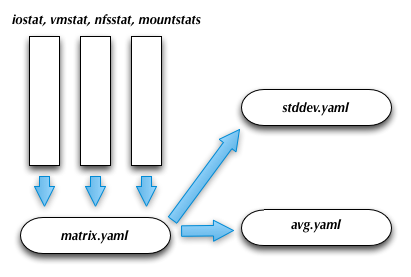
\includegraphics[height=6cm,width=11cm,scale=1.00]{/Users/yy/Pictures/final_paper/synthesis.png}
\caption{汇总及处理}
\label{}
\end{figure}
\end{frame}

\section{数据的比较分析及可视化}

\begin{frame}
\frametitle{数据比较分析}
已经可以进行的数据的比较和分析:
\begin{enumerate}
\item 比较多个commit
\item 比较多个config
\item 比较同一个config,commit的多次测试
\item 计算变化(包括上升和下降)的比例
\end{enumerate}

下面我们以vmstat和iostat这两个监视器中的两项指标进行比较分析(见下页)

\end{frame}

\begin{frame}
\frametitle{数据比较分析(续)}
\begin{figure}[htp]
\centering
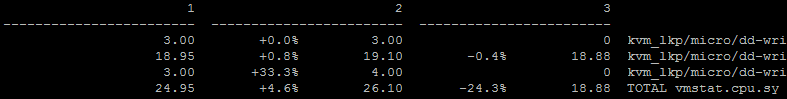
\includegraphics[height=2cm,width=11cm,scale=1.00]{/Users/yy/Pictures/final_paper/run_trim.png}
\caption{比较分析vmstat.cpu.sy}
\label{}
\end{figure}
\begin{figure}[htp]
\centering
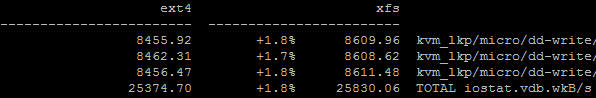
\includegraphics[height=2cm,width=11cm,scale=1.00]{/Users/yy/Pictures/final_paper/iostat_trim.png}
\caption{比较分析iostat.vdb.wkB/s}
\label{}
\end{figure}

\end{frame}

\begin{frame}
\frametitle{数据比较可视化}
根据前面的比较数据进行作图,方便比较:

\ 

\ 
\begin{minipage}[b]{0.48\linewidth}
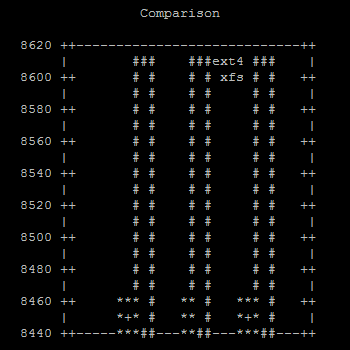
\includegraphics[height=4.8cm]{/Users/yy/Pictures/final_paper/iostat_fig.png}
\end{minipage}
\begin{minipage}[b]{0.48\linewidth}
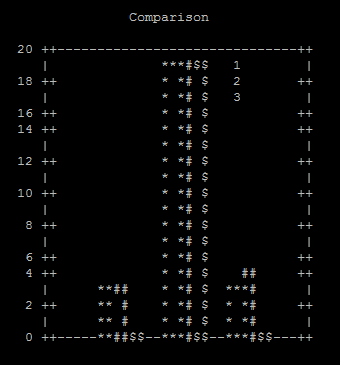
\includegraphics[height=4.8cm]{/Users/yy/Pictures/final_paper/run_fig.png}
\end{minipage}

\end{frame}


\section{Performance Regression判断算法}

\begin{frame}
\frametitle{简单算法}
在最初测试阶段,我们首先对某个指定的测试指标进行比较测试:
\begin{enumerate}
\item 只寻找regression(即下降)
\item 提供前后两个commit的某项测试数据
\item 预先对某一次的commit的相同config进行多次测试并记录测试数据
\item 人工分析历史数据确定偏离阈值
\end{enumerate}

在我们得到的数据中,我们可以获取任意一次测试的离散时间点上的所有监视数据,这里我们只是用整个测试过程中的监视指标平均值进行比较。

\end{frame}

\begin{frame}
\frametitle{简单算法存在的问题及优化思路}
\begin{block}{存在问题}
\begin{enumerate}
\item 有时是patchset出现问题而不是单个patch出现问题,此时应该挑出整段的patch而不是几个独立的patch
\item 阈值由人工指定,当比较的指标增多时,工作量比较大
\item 不同的config的阈值可能不同
\end{enumerate}
\end{block}
\begin{block}{优化思路}
\begin{enumerate}
\item 连续commit造成的问题在10-bisect递归算法中解决
\item 在相同config的前提下,利用所有正常的历史测试数据,作标准差$\sigma$,取阈值
$$threshold = k \sigma$$
使得我们能有较高的置信度(k=3时,置信度为99.7\%)
\end{enumerate}
\end{block}
\end{frame}


\section{下一步工作}

\begin{frame}
\frametitle{下一步工作}
中期之后马上将要展开的工作:
\begin{enumerate}
\item 根据数据进一步修改参数使得性能下降的判断算法能够更好地工作
\item 实现10-bisect搜索算法
\end{enumerate}

\end{frame}


\frame{
\center \huge \bfseries \color{red} Thank you!\\Q\&A?

}

\end{document}